\chapter{Synchronizing}

Synchronization refers to coordinating the actions of multiple processes that share resources.

In short, it involves the coordination of processes that access shared resources
\begin{itemize}
   \item Needs for avoiding inconsitencies or conflicts
   \begin{itemize}
      \item Prevent conflicts and inconsistencies that
      arise when multiple processes access
      shared data or resources concurrently.
   \end{itemize}
   \item Managing access to shared resources
   \begin{itemize}
      \item In a way that maintains data integrity and
      system performance.
   \end{itemize}
\end{itemize}

In Distributed Systems the communication happens through networks and message passing among multiple independent proceses.
\labelitemize{Challenges}{
   \begin{enumerate}
      \item Network Delays - Variable communication times may lead to inconsistencies
      \item Process Failures - Processes may fail at any time, so their failure must be handled
      \item No Fairness - We must preventing starvation or indefinite delays for processes waiting to access resources.
   \end{enumerate}
}

\section{Mutual Exclusion}
Mutual exclusion is a well-known \textbf{solution} to access shared resources in a distributed system, avoiding interferences.

\begin{definition}
   [Mutual Exclusion]
   A property that ensures only one process can enter a critical section at any given time.
\end{definition}
The \textbf{Critical section} is a portion of code accessing shared resources.

In other words, Mutual Exclusion enforces \textbf{atomical} access to shared resources, avoiding conflicts and inconsistencies.
Note that \textit{atomic} does not imply the hardware support for atomic operations, we use it as a logical and semantical concept.

\framedt{Mutual Exclusion Goals}{
   \begin{itemize}
      \item \textbf{Safety} - Only one process can access the critical section at a time
      \item \textbf{Liveness} - Ensures that every process that wishes to enter the critical section will eventually be able to do so, preventing starvation.
      \item \textbf{Fairness} - Requests for entry to the critical section are granted in the order they are made, ensuring no process is perpetually denied access.
   \end{itemize}
}


\subsection{Types of Mutual Exclusion}
\begin{enumerate}
   \item \textbf{Software-based} - Algorithms such as Lamport's Bakery Algorithm, Peterson's Algorithm, Dekker's Algorithm, etc.
   \item \textbf{Hardware-based} - Atomic operations or locks
   \item \textbf{Hybrid approaches} - Combining software and hardware-based solutions to achieve better performance and reliability.
\end{enumerate}

\begin{figure}[htbp]
   \centering
   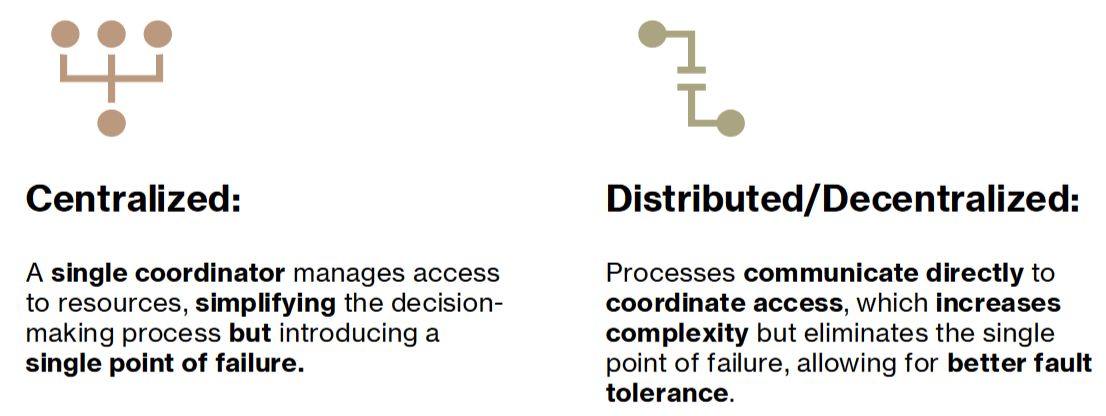
\includegraphics{images/04/mutual_types.png}
   \caption{Mutual exclusion - Centralized vs Distributed}
   \label{fig:04/mutual_types}
\end{figure}

\subsection{LBA - Lamport's Bakery Algorithm}
LBA is a software-based mutual exclusion algorithm that uses a ticket system to ensure fairness and prevent starvation.
LBA simulates a bakery where customers take a number and are served in order, clearly the processes are the customers.

\begin{enumerate}
   \item A process picks a ticket number that is one greater than the maximum ticket number currently in use.
   \item The process waits until all processes with smaller ticket numbers have completed their critical sections.
   \item The process with the lowest ticket number enters the critical section.
   \item The process resets its ticket number to indicate it has finished.
\end{enumerate}

It is \textbf{unlikely} for two processes to pick the same ticket number due to the sequential nature of ticket assignment, but it is possible.

In the rare cases where multiple processes attempt to obtain a ticket simultaneously, they may end up with the same number. To solve this the algorithm specifies that the process with the smaller identifier (\texttt{pid}) has priority ensuring fairness among competing processes.

The process enters the critical section only after verifying that no other process with a smaller ticket number is currently in the critical section.
Once the process completes its operations in the critical section, it releases its ticket by resetting its number to zero. The reset indicates to other processes that the critical section is available.

\begin{lstlisting}[language=C]
   choosing[N] -> {false, false, ..., false} // Initialize choosing flags for each process
   number[N] -> {0, 0, ..., 0} // Initialize ticket numbers for each process
   ...
   Process (i):
      lock(i);
         critical session code
      unlock(i);

   void lock(int i) {
      choosing[i] = true;
      number[i] = 1 + max(number[0], ..., number[N-1]);
      choosing[i] = false;
      for (int j = 0; j < N; j++) {
         while (choosing[j]); // Wait until other processes have chosen
         while (number[j] != 0 && (number[j] < number[i] || (number[j] == number[i] && j < i)));
      }
   }
\end{lstlisting}

Note that unlike some hardware-based synchronization mechanisms (like spinlocks or test-and-set instructions), LBA does not require atomic operations or specific CPU instructions. Besides, LBA relies on simple ticketing logic and does not depend on hardware features, it can be implemented in various environments, enhancing its portability.

Its major \textbf{drawback} is that it may suffer from performance issues (e.g., high communication overhead) in large systems due to continuous polling of ticket values.
However, it nicely environments where shared memory is available and the number of processes is relatively small.

\subsection{LDMEA - Lamport's Distributed Mutual Exclusion Algorithm}
LDMEA is a distributed version of Lamport's Bakery Algorithm that allows processes to access shared resources across multiple nodes, exploiting logical clocks for coordination.

\begin{figure}[htbp]
   \centering
   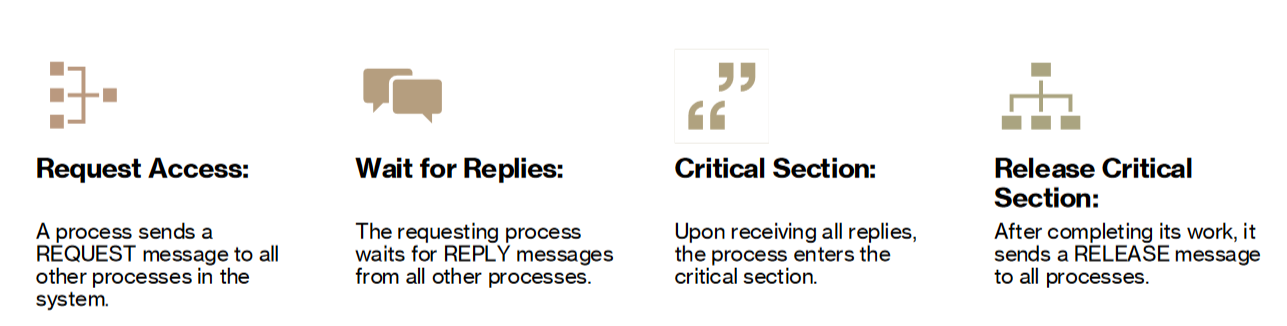
\includegraphics{images/04/ldmea_steps.png}
   \caption{LDMEA Key Steps}
   \label{fig:04/ldmea_steps}
\end{figure}

Each process maintains a logical clock to timestamp its requests, which is incremented at each request or receive.
Requests are ordered based on their logical timestamps, and the process with the smallest timestamp is granted access to the critical section.

Every site $S_i$, keeps a queue to store critical section requests ordered
by their timestamps. $request\_queue_i$ denotes the queue of site $S_i$.

\subsubsection{Entering the Critical Section}
When a site $S_i$ wants to enter the critical section, it sends a request message $Request(Ts_i, i)$ to all other sites and places the request on $request\_queue_i$. Here, $Ts_i$ denotes the timestamp of Site $Si$.
A site $S_i$ can enter the critical section if it has received the message with timestamp larger than $(ts_i, i)$ from all other sites and its own request is at the top of $request_queue_i$

\subsubsection{Leaving the Critical Section}
When a site $S_i$ leaves the critical section, it removes its own request from the top of its request queue and it sends a release message $Release(Ts_i, i)$ to all other sites and removes its request from $request_queue_i$.

When a site $S_j$ receives the timestamped RELEASE message from site $S_i$, it removes the request of $S_i$ from its request queue.

\subsubsection{Considerations and drawbacks}
\labelitemize{Example}{
   \begin{enumerate}
      \item \textbf{P1} sends a \texttt{REQUEST} message with its
      timestamp to \textbf{P2} and \textbf{P3}.
      \item \textbf{P2} and \textbf{P3} reply to \textbf{P1}.
      \item Once \textbf{P1} receives all \texttt{REPLY} messages, it
      enters the critical section.
      \item After finishing, \textbf{P1} sends a \texttt{RELEASE}
      message to \textbf{P2} and \textbf{P3}
   \end{enumerate}
}

Wrapping up we need
\begin{itemize}
   \item (N - 1) request messages
   \item (N - 1) reply messages
   \item (N - 1) release messages
\end{itemize}
So, the first drawback is that LDMEA incurs a high number of messages ($3n$) for each entry into the critical section. 
Besides, LDMEA also has to handle \textbf{failures}: requires additional mechanisms to handle process failures and network partitions.

However, the message passing in LDMEA, aside from making it suitable for distributed systems, even though it introduces overhead, it is still better than the polling mechanism in LBA, where processes have to continuously check for ticket values.

\subsection{Other approaches}
Lamport LBA and LDMEA are just two examples of mutual exclusion algorithms. There are many other algorithms that provide mutual exclusion in distributed systems, each with its own strengths and weaknesses.

Typically they are classified in three categories:
\begin{enumerate}
   \item Token-based algorithms
   \item Non token-based algorithms
   \item Quorum-based algorithms
\end{enumerate}

\newpage
\section{Token-based Algorithms}
A Token-Based Approach is a method used in distributed systems to manage access to a critical section. In this approach, \ul{a \textbf{unique token} circulates among the processes. Only the process that holds the token is allowed to enter the critical section}, ensuring \textbf{mutual exclusion}.

\paragraph*{Advantages}
\begin{itemize}
   \item \textbf{Efficiency} - When the token is well-managed, the system operates efficiently.
   \item Low Communication \textbf{Overhead} - There is minimal communication overhead when there is no contention for the token.
\end{itemize}

\paragraph*{Drawbacks}
\begin{itemize}
   \item Vulnerability to \textbf{Token Loss} - If the token is lost, it can disrupt the entire system.
   \item Token Circulation \textbf{Delays} - Delays in token circulation can lead to inefficiencies and increased waiting times for processes.
\end{itemize}

\subsection{Suzuki-Kasami Algorithm}
The process holding the token has exclusive access to the critical section. Request messages are sent to all processes when a process wants to enter.\\
Keep in mind that Suzuki-Kasami \ul{does \textbf{not} exploit logical clocks}. 

\framedt{Scenario}{
\begin{itemize}
   \item P1 wants to enter the critical section.
   \item It sends a request to all other processes.
   \item If it holds the token, it enters the critical
   section.
\end{itemize}
}

\subsubsection{Data Structures}
Each \textbf{process} maintains one data structure:
\begin{itemize}
   \item An array \lstinline|RN_i[N]|(for Request Number), \lstinline|i| being the \lstinline|ID| of the process containing this array, where \lstinline|RN_i[j]| stores the last Request Number received by \lstinline|i| from \lstinline|j|
\end{itemize}

The \textbf{token} contains two data
structures:
\begin{itemize}
	\item An array \lstinline|LN[N]|(for Last request Number), where \lstinline|LN[j]| stores the most recent Request Number of process \lstinline|j| for which the token was successfully granted
	\item A queue \lstinline|Q|, storing the \lstinline|ID| of processes waiting for the token
\end{itemize}

\subsubsection{Algorithm}
\paragraph*{Requesting the CS}
When process \lstinline|i| wants to enter the CS, if it does not have the token, it:
\begin{itemize}
	\item increments its sequence number \lstinline|RN_i[i]|
	\item sends a request message containing new sequence number to all processes in the system
\end{itemize}

\paragraph*{Releasing the CS}
When process \lstinline|i| leaves the CS, it:
\begin{itemize}
	\item Sets \lstinline|LN[i]| of the token equal to \lstinline|RN_i[i]|. This indicates that its request \lstinline|RN_i[i]| has been executed.
	\item for every process k not in the token queue \lstinline|Q|, it appends \lstinline|k| to \lstinline|Q| if \lstinline|RN_i[k] == LN[k]+1|. This indicates that process \lstinline|k| as a pending request
	\item if the token queue \lstinline|Q| is not empty after this update, it pops
   a process ID \lstinline|j| from \lstinline|Q| and sends the token to \lstinline|j|
	\item otherwise, it keeps the token
\end{itemize} 

\paragraph*{Performance}
\begin{itemize}
	\item Either 0 or N messages for CS invocation (no messages if process holds the token; otherwise N-1 request and 1 reply)
	\item Synchronization delay is 0 or N (N-1 requests and 1 reply)
\end{itemize}


The main two \textbf{issues} are discerning \textbf{outdated requests} from current ones, and determining which site is going to get the token next.
Besides, if a token is lost, processes can hang; token recovery mechanisms or
timeout strategies may be implemented to handle token loss.


On the other hand it is \textbf{efficient} in terms of message passing, as it only requires up to N messages for each CS invocation, and the synchronization delay is is 0 or N (N-1 requests and 1 reply).
It suits high-latency networks.



\section{Non-token-based Algorithms}

Processes communicate directly with each other to request permission to enter the critical section.
There is \textbf{\textit{no} central authority} or \textbf{token}, and there are messages exchanged to determine access rights.

\subsection{Ricart-Agrawala Algorithm}
\label{sec:04/ricart_agrawala}
Its goal is to achieve mutual exclusion by having processes send requests to each other: a process sends a request message to all other processes, waiting for replies to enter the critical section.

All processes communicate directly without a token in a decentralized fashion, and for each request $2(N-1)$ messages are exchanged.

\textbf{Fairness} is enforced by the timestamping mechanism, where the process with the smallest timestamp has priority: requests are served based on the order of arrival, governed by logical timestamps. If two processes have the same timestamp, the process with the lower ID gets priority.

Considering the previous points, the Cons are that message passing is high, and the algorithm is not suitable for high-latency and unreliable networks.

\section{Quorum-based Algorithms}

Instead of communicating with all processes, a process communicates with only a subset (quorum) of processes to get permission to enter the critical section.

\subsection{Maekawa's Algorithm}
A \textbf{quorum} is a subset of processes that must grant
permission for mutual exclusion.
Ensures that any two quorums overlap, guaranteeing access.

It has a reduced number of messages compared to the Ricart-Agrawala (Sec. \ref{sec:04/ricart_agrawala} algorithm, and fits nicely environments with many \textbf{processes} and \textbf{high contention}.

\section{Wrap Up}

\begin{figure}[htbp]
   \centering
   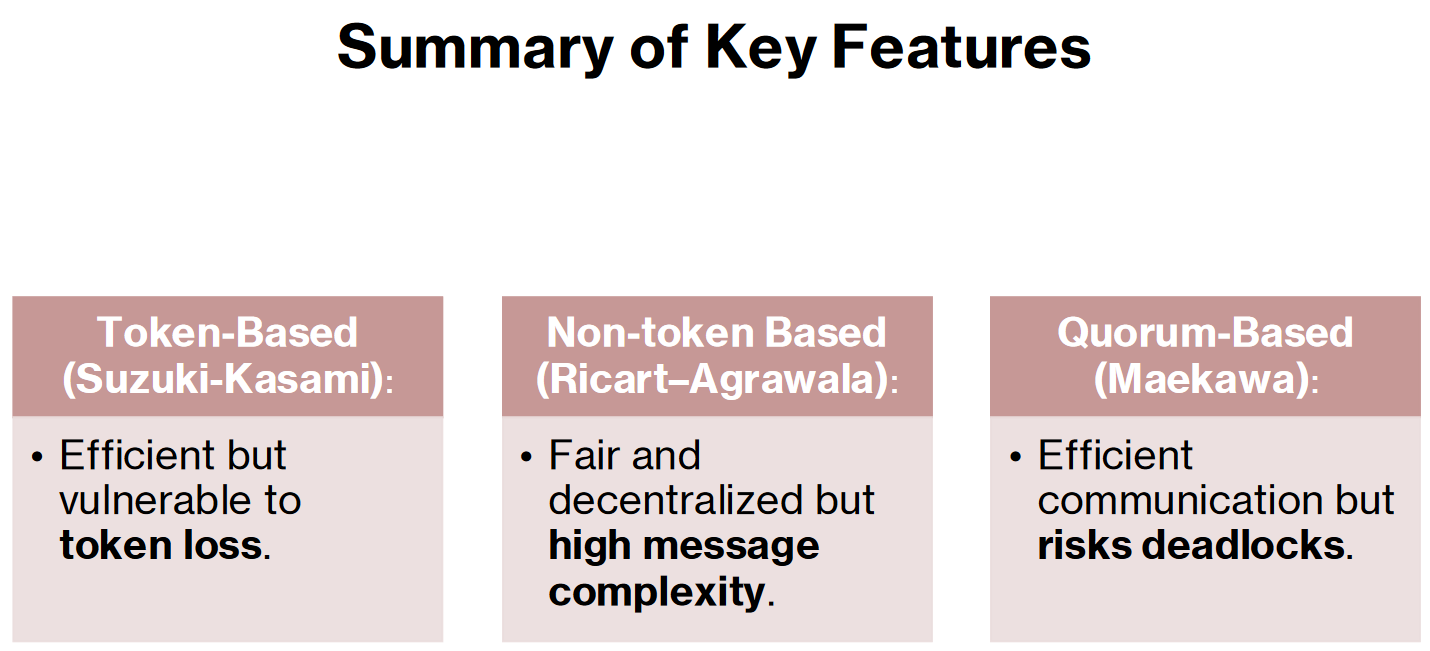
\includegraphics{images/04/wrapup_key.png}
   \caption{Summary of the Key features}
   \label{fig:04/wrapup_key}
\end{figure}

\paragraph*{Message complexity}
Message Complexity:
\begin{itemize}
	\item \textbf{Suzuki-Kasami} - Low message overhead during token passing.
	\item \textbf{Ricart-Agrawala} - High message complexity due to multiple
requests and replies.
	\item \textbf{Maekawa} - Reduced message count by only requiring
quorum approval.
\end{itemize}

\paragraph*{Scalability Considerations}

\begin{itemize}
   \item \textbf{Token}-Based - Scales well with fewer processes; token management becomes complex as the number of processes increases.
   
   \item \textbf{Non-token} Based - Scalability issues arise with an increasing number of processes due to high message overhead.
   
   \item \textbf{Quorum}-Based - Efficient for many processes, but the quorum size must be managed carefully to avoid performance degradation.
\end{itemize}

\paragraph*{Potential Strategies}

\begin{itemize}
	\item \textbf{Suzuki-Kasami} - Implement token recovery mechanisms to recreate lost tokens.
	\item \textbf{Ricart-Agrawala} - Use timeouts to handle unresponsive processes.
	\item \textbf{Maekawa} - Adjust quorum sizes dynamically based on active processes.
\end{itemize}

\paragraph*{Takeaway}

\begin{itemize}
	\item \textbf{Suzuki-Kasami} - Efficient token management but vulnerable to loss.
	\item \textbf{Ricart-Agrawala} - Fairness and decentralization but high message complexity.
	\item \textbf{Maekawa} - Reduced communication overhead with quorum mechanisms but requires careful management to avoid deadlocks.
\end{itemize}